% \documentclass[10pt]{scrartcl}
\documentclass[10pt,twocolumn]{scrartcl}

\usepackage[utf8]{inputenc}
\usepackage[T1]{fontenc}
\usepackage[ngerman]{babel}

\usepackage{amsmath}
\usepackage{amssymb}

\usepackage{graphicx}
\usepackage{tabularx}

\setlength{\parindent}{0cm}
\setlength{\parskip}{3mm}
\setlength{\textheight}{23.8cm}
\setlength{\headheight}{1cm}
\setlength{\topmargin}{-10mm}

\setlength{\oddsidemargin}{0cm}
\setlength{\evensidemargin}{0cm}
\setlength{\textwidth}{16cm}
\setlength{\columnsep}{8mm}

\usepackage{multicol}
\usepackage{colortbl}
\usepackage{xcolor} 
\usepackage[hyphens]{url}
\definecolor{grau}{gray}{0.95}
\definecolor{dunkelgrau}{gray}{0.85}

\usepackage[normal]{caption}
\usepackage{lipsum}

\setlength{\parindent}{5mm}
\setlength{\parskip}{0mm}

\usepackage{float}
\restylefloat{figure}

\renewcommand{\topfraction}{0.75}
\renewcommand{\textfraction}{0.2}

%###########################################################
% die Sachen mit der Kopfzeile
\usepackage{lastpage}
\usepackage{fancyhdr}
\fancyhf{} % leere alle Felder
\fancyhead[R]{\footnotesize Marvin Klose, Michael Josef Wieneke\\ Inga Miadowicz}
\fancyhead[L]{\footnotesize Ausgewählte Methoden der
Datenanalyse, \\ Modellierung und Simulation} % Titel des Aufsatzes
\fancyfoot[C]{\footnotesize \thepage/\pageref{LastPage}}
% \fancyfoot[C]{\footnotesize \thepage}
\renewcommand{\headrulewidth}{0.4pt} % obere Trennlinie
\pagestyle{fancy}
%###########################################################

\newcommand{\ownsection}[1]{\begin{center}\LARGE\bf#1\end{center}}

\begin{document}

\twocolumn[
\ownsection{Ausbreitung von Infektionskrankheiten innerhalb einer Population}

\begin{center}
Inga Miadowicz (Inga.Miadowicz@gmx.de) \\
Marvin Klose (Marvin.Klose@sap.com) \\
Michael Josef Wieneke (Michael.Wieneke@sap.com)\\
Mannheim, November 2014
\end{center}
\vspace*{5mm}
]

\section*{Abstract}
Jährlich sterben Millionen von Menschen an den verschiedensten Krankheiten. Sie infizieren dabei sich durch Übertragungswege wie Tröpfchen, Kontakt, Lebensmittel oder Trinkwasser. Medikamente und Therapien gibt es für fast alle bekannten Krankheiten, dennoch gibt ist Krankheiten mit tödlichem Ausgang. Deshalb ist interessant zu beobachten, wie sich Krankheiten unter bestimmten Parametern ausbreiten und wie Faktoren wie Resistenzen den Verlauf verändern können. Um schon möglichst präventiv Maßnahmen treffen zu können, damit erst gar keine Pandemie ausbricht und die Zahl möglicher Todesopfer zu minimieren. Der aktuellste Fall einer solchen akuten Bedrohung ist Ebola, welches momentan noch hauptsächlich in Westafrika auftritt. Dieses Themengebiet is nicht nur in der Biologie relevant, sondern lässt auch auf die Informatik übertragen. Computer können sich über Netzwerke und das Internet ebenfalls mit solche Viren oder Würmern anstecken. Dies ist jedoch nicht Bestand der Ausarbeitung.

\section*{Einleitung}

Die hier vorgestellte Ausarbeitung entstand im Rahmen der Vorlesung \glqq Ausgewählte Methoden der Datenanalyse, Modellierung und Simulation\grqq\; an der Dualen Hochschule Baden-Württemberg.
In der Vorlesung wurde ein Modell entwickelt, mit dem Ziel die Ausbreitung von Infektionskrankheiten zu simulieren.
Zentrale Aspekte sind deshalb die Gesundheit der Bevölkerung und die Veränderungen der Bevölkerungszahl, aufgrund von Epidemien. Somit lässt sich das Thema wissenschaftlich unter dem Begriff der Epidemiologie einordnen.
Dass das Thema nach wie vor Relevanz hat, sieht man an der aktuellen Ebola Epidemie, die sich hauptsächlich in Afrika ausbreitet. Zudem haben auch schon in der Vergangenheit immer wieder Epidemien Aufsehen erregt. Darunter beispielsweise 2006 die Vogelgrippe  \cite{gehlhoff2007chronik}
oder 2000/2001 BSE \cite{Spon:2014}. Diese forderten jedoch im Vergleich zur spanischen Grippe, die mehrere Millionen Menschen das Leben kostete, vergleichsweise wenig Todesopfer. Die spanische Grippe war die bisher verheerendste Influenzapandemie und forderte etwa 50 Millionen Todesopfer \cite{welt:2014}. Zusätzlich spricht man bei HIV/AIDS ebenfalls von einer Pandemie bei der nach Angaben der Organisation UNAIDS seit Bekanntwerden der Krankheit zwischen 35 und 43 Millionen Menschen gestorben sind  \cite{UNAIDS:2014}.
Damit ist ein Ziel des Modells die bestmöglichen Gegenmaßnahmen zu treffen, um die Bevölkerung zu schützen und so die Anzahl der Todesopfer zu minimieren.
Das vorgestellte Modell simuliert dazu die Entwicklung verschiedener Krankheiten innerhalb einer Population über einen gewissen Zeitraum. 
\smallskip

Inhaltlich beginnen wir mit der Erläuterung bestehender Modelle der Wissenschaft. Anschließend folgt die Vorstellung des von uns entwickelten Modells, das wir im Anschluss daran mit SIR-Modell vergleichen wollen. Darauf folgen die Ergebnisse und eine Diskussion. Abschließend gibt es einen Ausblick, der mögliche Erweiterungen unseres Modells behandelt. 


\subsection{Modelle in der Wissenschaft}
Ein Ansatz zur mathematischen Betrachtung der Krankheitsausbreitung ist das SIR-Modell von William O. Kernack und Anderson Gray McKendrick.\\
Es ist 1927 mit dem Zweck die Verbreitung Krankheiten sowie den Folgen von Gegenmaßnahmen von gesundheitsbezogenen Zuständen und Ereignissen in Bevölkerungen oder Populationen zu untersuchen.\\
In diesem Abschnitt wird zunächst die Idee hinter dem SIR-Modell vorgestellt, dann die Mathematik hinter dem SIR-Modells erklärt und abschließend aufbauend darauf die Frage beantwortet, warum gerade dieses Modell für den Vergleich des Projektes mit bekannten Methoden aus der Wissenschaft gewählt wurde.
\subparagraph{Theorie des SIR-Modells}
\begin{figure}
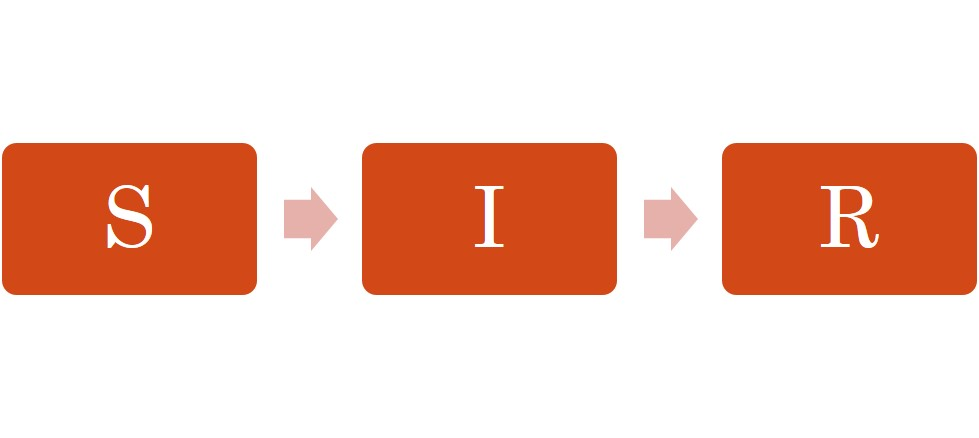
\includegraphics[width= 0.3\textwidth]{./images/SIR-Modell.jpg}\caption{Zustandsmodell des SIR-Modells}\label{fig:SIR}
\end{figure}
Das SIR-Modell ist eine mathematische Herangehensweise, bei der der Krankheitsverlauf statisch über feste Funktionsterme errechnet wird. \\
Dazu wird eine geschlossene Gruppe \textbf{N} an Individuen betrachtet. Die Anzahl \textbf{N} ist die Gesamtgröße der Bevölkerung. Die Bevölkerung setzt sich aus gesunden, kranken und \glqq R\grqq-Individuen zusammen, sodass gilt:
\begin{equation}\label{eq:N}
N = S + I + R
\end{equation}
Das heißt, die Bevölkerung wird in drei Zuständen klassifiziert:
\begin{itemize}
\item \textbf{S (Susceptible)} Anfällige Individuen, die innerhalb der Bevölkerung Infiziert werden können.
\item \textbf{I (Infected)} Infizierte Individuen, die Anfällige anstecken  oder in den \glqq R\grqq -Zustand übergehen können.
\item \textbf{R (Recovered)} Individuen im \glqq R\grqq -Zustand. Ein infiziertes Individuum, was in den \glqq R\grqq -Zustand übergeht, bleibt im R-Zustand. Es gibt keinen Übergang aus dem \glqq R\grqq -Zustand zurück in einen der anderen Zustände. Der \glqq R\grqq -Zustand kann von daher Individuen beschreiben, die aus Epidemiologischer Sicht keinen Einfluss mehr auf den Rest der Gesellschaft haben. Dies könnten z.B. immunisierte, tote oder isolierte Personen sein.
\end{itemize}
Das Bild \ref{fig:SIR} zeigt das entsprechende Zustandsübergangsmodell zu den drei Bevölkerungsgruppen.\\
Zur Visualisierung des Krankheitsverlauf in einer Bevölkerung kann geeigneter Weise ein Koordinatensystem benutzt werden, dass die Anzahl der Individuen in Relation zur Zeit setzt.
Für jede Zustandsgruppe wird ein Graph in das Koordinatensystem gezeichnet, sodass ablesbar wie viele Individuen zu einem Zeitpunkt krank, gesund oder im \glqq R\grqq-Zustand sind.\\
Die Verteilung der Individuen in die jeweiligen Zustandsklassen ändert sich mit dem Fortschritt der Zeit \textbf{t}, ist die Krankheit nicht ausgestorben, die Infektionsrate oder \glqq R\grqq-Übergangsrate größer null und nicht alle Individuen im \glqq R\grqq-Zustand.
Für jeden Zeitschritt wird die Anzahl der Individuen in den Zustandsklassen neu berechnet.\\
Beispielsweise könnten nach einem Zeitschritt drei neue Individuen erkranken und ein Mensch stirbt. Damit nimmt die Gruppe  \textbf{S} um drei Individuen ab, die Gruppe \textbf{I} wächst entsprechend um drei und gibt gleichzeitig ein Individuum an die Gruppe \textbf{R} ab, sodass sich die Verteilung nach einem Zeitschritt wie in Bild \ref{fig:sch} ändert.
\subparagraph{Berechnung der Entwicklung mit dem SIR-Modell}
\begin{figure}
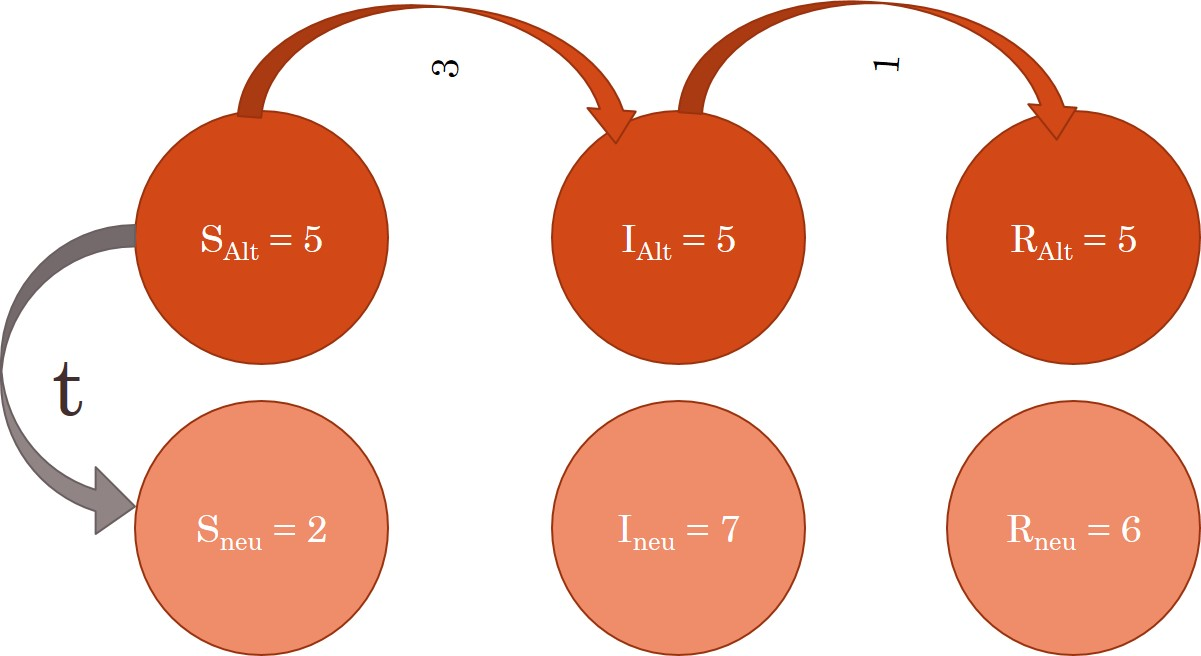
\includegraphics[width= 0.3\textwidth]{./images/SIR-Berechnung.jpg}\caption{Möglicher Zustandswechsel nach einem Zeitschritt}\label{fig:sch}
\end{figure}
Damit die Verteilung sinnvoll berechnet werden kann, werden Kennzahlen über die Krankheit benötigt, die das Krankheitsprofil widerspiegeln. Dabei wird für das SIR-Modell die Infektionsstärke und die \grqq R\glqq{}-Übergangsrate benötigt.
Über die Infektionsstärke $\lambda$ wird die Ansteckung-Kontakt-Rate \textbf{b} ermittelt \ref{eq:b}. Diese ist die Wahrscheinlichkeit mit der ein Individuum, dass mit \textbf{X} Individuen pro Zeitschritt Kontakt hat, erkranken kann.
\begin{equation} \label{eq:b}
b = ( \lambda * X ) / N
\end{equation}
Dabei ist die Anzahl X der Kontakte pro Zeiteinheit je nach Krankheitsübertragungsweg zu unterscheiden. Bei Krankheiten die über Tröpfcheninfektion übertragen werden, reicht Hände schütteln, die Übergabe von Geld oder sogar das Zusammensein in einem Raum zur Infektion. In diesem Szenario wird ein Durchschnittswert von 8 Menschen am Tag genommen.
Bei Krankheiten mit anderen Übertragungswegen z.B. AIDS muss der Austausch von Körperflüssigkeiten zur Infektion stattfinden, d.h. \textbf{X} zeigt den durchschnittlichen Austausch von Körperflüssigkeiten in einem Zeitabschnitt. In diesem Fall ist \textbf{X} im Durchschnitt natürlich deutlich geringer als bei Tröpfcheninfektion.\\
Über die Ansteckungs-Kontakt-Rate kann die Basisreproduktionsrate \ref{eq:R0} ermittelt werden. Diese beschreibt die Anzahl der Erwarteten Ansteckungen durch einen zusätzlichen Infizierten.
\begin{equation}\label{eq:R0}
R_0 = \frac{ b * N }{ \gamma }
\end{equation}
Hat man die beiden Größen ermittelt, können die Funktionen für die drei Zustände S, I und R über einen Zeitraum ermittelt werden. 
Es gilt:
\begin{equation}
\frac{ \delta S }{ \delta t } = -R_0 \cdot \frac{S * I}{N}
\end{equation}
Die erwartete Anzahl an Neuinfizierungen mal den Anteil der Gesunden und Infizierten Individuen von der Gesamtbevölkerung, ergibt die Anzahl der Gesunden, die diese Runde Infiziert werden. Die Menge der Anfälligen wird um die Menge der Neuinfizierten reduziert.
\begin{equation}
\frac{\delta I }{\delta t} = R_0 \cdot \frac{S \cdot I}{N}
\end{equation}
Diese Funktion berrechnet die Anzahl der Neuinfizierten von der Menge der Infizierten und der Anfälligen. Die Menge der Infizierten I wächst um die Menge der Anfälligen, die sich diese Runde infiziert haben.
\begin{equation}
\frac{\delta R }{\delta t} = \gamma \cdot I
\end{equation}
Die Anzahl der Individuen im R-Zustand wächst um einen Anteil $\gamma$ von den Infizierten. Das Heißt Einige Infizierte werden der Menge I abgeführt und wandern in Zustand R über. Von diesem Überstand ist kein anderer Zustand erreichbar, d.h. Diese Menge wächst stetig wenn $\gamma$ 0 und die Baisisreproduktionsrate größer null sind.

\subparagraph{Wahl des SIR-Modells als Referenzmodell}
\begin{figure}
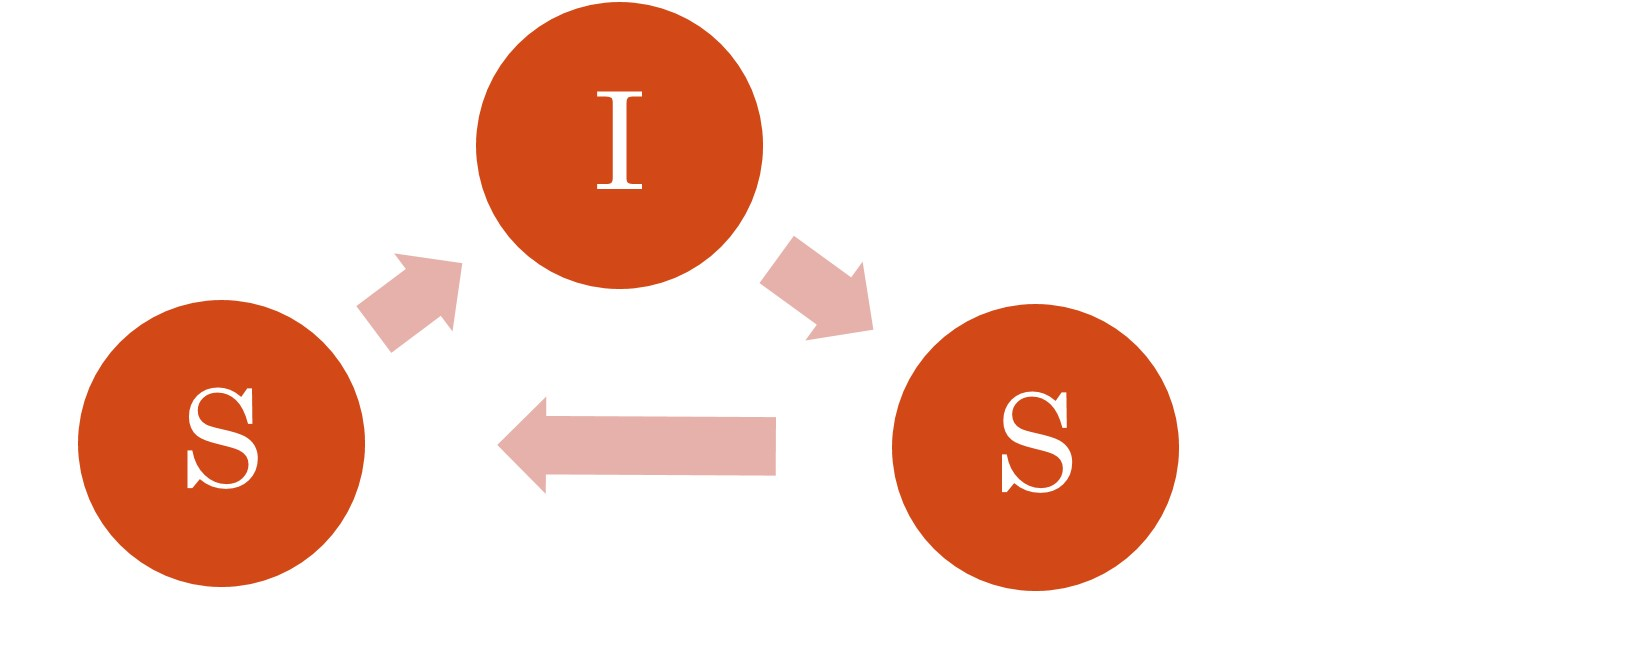
\includegraphics[width= 0.3\textwidth]{./images/SIS-Modell.jpg}\caption{Zuständsmodell des SIS-Modells}\label{fig:sis}
\end{figure}
Bei dem Vergleich mit bekannten Modellen aus der Wissenschaft drängt sich zunächst die Frage auf warum im Rahmen des Projektes gerade der Vergleich mit dem SIR-Modell angestellt wird und nicht mit einem anderen Modell zur Darstellung eines Krankheitsverlauf.\\
Wie genau ein mathematisches Modell die Krankheitsausbreitung in einer Gesellschaft beschreibt, hängt sehr davon ab, wie viel Realismus und damit wie viele Annahmen hineingesteckt werden.\\
Da in der Medizin viele Einflüsse zunächst vernachlässigt werden müssen, nicht bekannt sind oder die Krankheit sich mit der Zeit durch mutierende Viren verändert, haben die Modelle sehr selten einen endgültigen Charakter. Darüber hinaus sind Krankheiten in ihrer Entwicklung so unterschiedlich, dass es sehr oft möglich und manchmal nötig ist, die Modelle weiter zu verfeinern und anzupassen, wobei unterschiedliche Krankheiten unterschiedliche Modelle erfordern können. 
\cite{sebM}\\
Mit anderen Worten: Eine Krankheit kann mit all ihren Eigenschaften sehr realitätsnah abgebildet werden, aber möglicherweise bei einer anderen Krankheit schon wieder versagen. Von daher ist nicht das Modell, sondern das zugrunde liegende Szenario entscheidend für die Wahl des Vergleichsmodells. Eine sinnvolle Vorgehensweise ist es daher erst ein Szenario zu erschaffen und dieses dann mit einem geeigneten Modell abzubilden.\\ 
Im Rahmen unserer Projektes wurde sich für die Mittelalterpest entschieden.\\ 
Die Mittelalterpest war im 14. Jahrhundert gleichzusetzen mit einem Todesurteil. Beinahe jedes Individuum erlag nach einiger Zeit seiner Krankheit. Aus diesem Grund passt die Natur des Modells sehr gut zum vorgegebenen Szenario und dem Krankheitsprofil der Pest: Ein gesundes Individuum kann infiziert werden und dann sterben. In diesem Fall bildet der \glqq R\grqq-Zustand, die Anzahl der verstorbenen Individuen ab.\\
Mit einem anderen Szenario wäre es sinnvoll gewesen ein anderes Modell zu betrachten. 
Andere Modelle, die in der mathematischen Biologie angewendet werden sind z.B. das SI-Modell oder SIS-Modell.\\
Das Zustandsmodell im SIS-Modell ist im Gegensatz zum SIR-Modell zyklisch. Es gibt nur zwei Zustände: Anfällig und Infiziert. Anfällige Individuen können infiziert werden und dann wieder genesen und sich erneut infizieren, wie im Bild \ref{fig:sis}. Sind sie genesen können sie wiederum infiziert werden. Damit ist das SIS-Modell vor allem geeignet für bakterielle Erkrankungen wie z.B. Tuberkulose, bei der Individuen wieder genesen, aber keine Immunität entwickeln. \\
Das SI-Modell hat ebenfalls die beiden Zustände Anfällig und Infiziert, aber ist nicht zyklisch. Es können lediglich Individuen Infiziert werden. Diese bleiben endgültig im Zustand I.\\ 
Das SI-Modell ist also sinnvoll, wenn Individuen lediglich an einer Krankheit erkranken und nicht wieder genesen, aber auch nicht sterben. Das entsprechende Szenario, wäre also ein Virus, der ein Individuum auf Lebzeiten oder sogar darüber hinaus. Ein mögliches Szenario wäre ein aus Hollywood bekanntes Filmszenario der berühmten Zombie-Apokalypse.\\
Damit wird der erste Vorteil der Herangehensweise im Programm sichtbar: Während bei der mathematischen berechnen für jede Infektionskrankheit ein anderes Modell gewählt werden muss, um möglichst nah an der Realität zu bleiben, ist das Programm auf mehrere Szenarien mit Heilung, Toten, Resistenten etc. anwendbar.
Wie bereits erläutert weißt das SIR-Modell einige Schwächen auf unter Anderem wird in dem Modell davon ausgegangen dass jeder Mensch im Schnitt acht Kontakte, je nach Modellierung, zu anderen Menschen hat. In unserem Programm wird dies dynamisch geregelt, dort gibt es einen Raster welcher einem Schachbrett ähnelt auf diesem beliebig großem rechteckigem \glqq{}Raster\grqq{} lassen sich an jeder $ x,y $ Position Zellen positionieren. So kann es Zellen geben welche sehr viele Nachbarn haben aber auch Zellen welche gar keinen Nachbar haben. Einen exemplarischen Raster sieht man in  Abbildung \ref{fig:Raster}. Auf diesem 3x3 Raster befinden sich aktuell drei Zellen theoretisch ist es aber auch möglich diesen Raster mit bis zu 9 Zellen zu besiedeln. So können auch extreme Situationen realistisch dargestellt werden wie zum Beispiel sehr dünn besiedelte Gegenden oder aber auch mittelalterliche Städte in denen in einem Haushalt durchaus 20 Personen lebten.\\

%Quelle recherchieren

\begin{figure}[t]
\centering
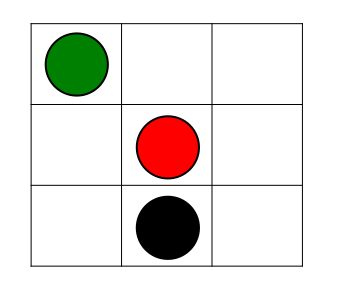
\includegraphics[width= 0.45\textwidth]{./images/nachbarn.png}
\caption{Ein 3x3 Raster mit Zellen in drei verschiedenen Zuständen}
\label{fig:Raster}
\end{figure}

\subsection*{Zelluläre Automaten}
Die vorliegende Implementierung basiert auf zellulären Automaten. Das heißt das jede Zelle erst einmal für sich unabhängig von anderen Zellen existiert.Eine Zelle ist im Kontext dieser Arbeit ein Mensch oder ein Tier. Dabei kann sich die Zelle in jeder Phase der Simulation nur in genau einem der folgenden Zustände befinden:
\begin{enumerate}
\item{\emph{Anfällig}\\
Eine anfällige Zelle kann nur von infizierten Zellen in ihrem direkten Umfeld welches durch eine Moore-Nachbarschaft \cite{Weisstein:2014} des Radius 1 charakterisiert wird angesteckt werden. Daraus folgt, dass eine Zelle auf dem rechteckigen Raster nur von den Zellen links über ihr, direkt über ihr, rechts über ihr, links und rechts neben ihr und links neben ihr, links unter ihr, direkt unter ihr und rechts unter ihr angesteckt werden kann.Dies sind im inneren des Spielfeldes maximal acht Zellen wie man am Beispiel der roten Zelle in Abbildung \ref{fig:Raster} gut sehen kann.\\
Des Weiteren wird auch betrachtet ob die Krankheit auch von jeder Zelle auf jede übertragbar ist oder ob zum Beispiel nur eine Übertragung von Mensch auf Tier aber nicht von Mensch auf Mensch möglich ist.\\
Angenommen die rote Zelle in Abbildung \ref{fig:Raster} ist ein infizierter Mensch und  die grüne Zelle ein gesundes Tier und die simulierte Krankheit lässt sich nicht von Mensch auf Tier übertragen. Demzufolge ist die grüne Zelle zu diesem Zeitpunkt vollkommen sicher, da sich in ihrer Nachbarschaft keine für sie potentiell gefährlichen Zellen befinden. 
}
\item{\emph{Infiziert}\\
Eine infizierte Zelle kann an ihrer Krankheit sterben, heilen und damit in den ersten Zustand übergehen, eine Resistenz bilden und damit in den dritten Zustand übergehen oder sie bleibt weiterhin infiziert.\\
All dies geschieht unter Berücksichtigung der für die simulierte Krankheit eingegebenen Werte.\\
Des Weiteren kann sie natürlich alle gesunden Zellen in ihrem Umfeld infizieren, auch dies geschieht unter Berücksichtigung der Werte die für die aktuelle Krankheit gelten.
}
\item{\emph{Resistent}\\
Da resistente Zellen nicht mehr in den Infiziert Zustand übergehen können und das Programm keine natürlichen Tode vorsieht, sind diese Zellen im Kontext des Programms unsterblich.\\
Sie werden jedoch trotzdem betrachtet, da sie im Kontext der Simulation interessant sind. So könnte man beispielsweise betrachten wie sich eine Krankheit verbreitet wenn bereits fast alle Zellen immun sind und es nur sehr wenige infizierte und anfällige Zellen gibt. Denkbar ist in diesem Szenario, dass die resistenten Zellen die infizierten Zellen weitestgehend abschirmen und so eine weitere Verbreitung verhindern. 
}

\item{\emph{Tot}\\
Eine Zelle in diesem Zustand, ist für die weitere Simulation nicht relevant. Naheliegenderweise kann sie sich nicht mehr eigenständig bewegen und auch kann sie keine anderen Zellen mehr infizieren. Es mag zwar durchaus Krankheiten geben welche auch nach dem Tot des Wirtes infektiös, an dieser Stelle wird in der Simulation davon ausgegangen dass die Zelle sich in einem intaktem Umfeld befindet in dem Tote entweder isoliert werden, dass sie keinen Kontakt mehr zu lebendigen Individuen haben. 
}
\end{enumerate}

\subsection*{Bewegung}
Zellen die sich in einem der ersten drei Zustände befinden können sich bewegen. Dabei wird in dieser Simulation davon ausgegangen dass die Zellen sich in einem geschlossenem Umfeld befinden. Es können also keine Zellen das Simulationsgebiert verlassen oder neu betreten.\\
Des Weiteren handelt es sich um eine zweidimensionale Simulation in der es nicht möglich ist dass sich mehrere Zellen auf einem Feld über- oder untereinander befinden.\\
Im allgemeinen Fall bewegen sich die Zellen dem Simple Isotropic  Random Walk Model \cite{Codling:2008} entsprechend, dies bedeutet dass sich eine Zelle zufällig in irgendeine Richtung bewegt unabhängig davon wohin sie sich zuvor bewegt hat. Dabei wird davon ausgegangen dass die Zellen grundsätzlich einen Drang zur Bewegung haben.\\
Sollte sich eine Zelle jedoch entscheiden sich in ein Feld zu bewegen indem schon eine andere Zelle ist, ist diese Bewegung nicht möglich und die Zelle muss sich neu entscheiden. Das Gleiche gilt für Zellen am Rand des Simulationsgebietes. Natürlich gibt es die Möglichkeit dass eine Zelle komplett \glqq umringt\grqq\; von anderen Zellen ist, in diesem Fall bleibt die Zelle zwangsweise an ihrer alten Position.\\
Veranschaulicht bedeutet dass das zum Beispiel die grüne Zelle in Abbildung \ref{fig:Raster} nur zwei Möglichkeiten hat sich zu bewegen. Nämlich eine Bewegung nach unten oder nach rechts. Da über und links neben ihr keine Felder mehr sind und auf der Diagonale kann sie sich auch nicht bewegen da dort die rote Zelle das einzig mögliche Feld blockiert.\\
%Quelle hier einbinden
\subsection*{Wirtsbeziehungen}
Die Simulation ist in der Lage einfache Wirtsbeziehungen zu simulieren, dadurch dass es zwei Arten von Zellen gibt (Menschen und Tiere), kann man krankheitsabhängig unterscheiden ob eine Krankheit jeweils von Mensch auf Mensch, von Mensch auf Tier, von Tier auf Mensch und von Tier auf Tier übertragbar ist, so kann schon eine beträchtliche Menge von Krankheiten simuliert werden.\\
Dies ermöglicht es zu simulieren was passiert wenn man versucht Krankheiten wie die Tollwut welche fast ausschließlich von Tieren auf den Mensch übertragen werden, versucht auszurotten indem man alle potentiellen Wirte immunisiert.

\subsection*{Bevölkerungsdichte}
Im Rahmen dieses Modell ist es möglich zu simulieren wie sich eine Krankheit bei verschiedener Bevölkerungsdichte verhält. So ist es möglich dass es auf einem gegebenem Raster $x\cdot y$ für die gilt $ x,y \in \mathbb{N}$ zwischen $1$ und $x\cdot y$ Zellen zu platzieren.\\
Dabei ist auch das Verhältnis von Menschen zu Tieren vollkommen beliebig wählbar. So lassen sich die Auswirkungen der Bevölkerungsdichte auf die Entwicklung simulieren.

\subsection*{Nicht deterministisch}
Ob eine Zelle in einen bestimmten Zustand übergeht hängt einerseits von ihrem eigenem Zustand und den Zuständen ihrer Nachbarn, andererseits von einer krankheitstypischen Wahrscheinlichkeit ab. Sollte eine Zelle infiziert sein und bei der simulierten Krankheit besteht die Wahrscheinlichkeit zu sterben bei 25\% so wird der Wert 0.25 mit einer zufälligen Zahl zwischen 0 und 1 verglichen. Sollte diese Zufallszahl größer sein als die Übergangswahrscheinlichkeit geht die Zelle in den entsprechenden Zustand über.\\
Das bedeutet das selbst wenn man die Simulation mit exakt den selben Parametern mehrmals durchführt man unterschiedliche Ergebnisse erzielen kann. Das Modell ist also nicht deterministisch.


%\begin{enumerate}
%\item{Bewegung}
%\item{\emph{Wirtsbeziehungen}
%
%
%
%}
%\item{\emph{Bevölkerungsdichte wird berücksichtigt}
%
%
%}
%\item{nicht deterministisch}
%\end{enumerate}


\section*{Vergleich mit dem SIR Modell}
Da die mathematische Beschreibung, sowie das Programm beide den Verlauf von Krankheiten simulieren, liegt ein Vergleich der beiden Herangehensweisen nahe. 
Dieser soll anhand eines konkreten Testszenarios angewandt werden, bei dem beide Modelle mit denselben Daten eine Prognose über die Entwicklung einer Krankheit liefern sollen.\\
Der Vergleich soll eine Einschätzung der Repräsentativität, des dem Projekt zugrunde liegenden Programms ermöglichen und Schwächen und Stärken der beiden Modelle herausstellen.\\
Dazu wird zunächst das Testszenario vorgestellt und dann in beiden Modellen angewandt.
Auf einer kurze Vorstellung der Ergebnisse in den Modellen folgt zu guter Letzt eine Gegenüberstellung der beiden Resultate.
Für die Visualisierung der Daten des SIR-Modells wurde im Nachfolgenden die SIR-Simulation von Hans Nesse benutzt.%\cite{XXX}

\subsection*{Szenario}
Das Testszenario spielt in einem kleinen Dorf mit 10150 Einwohnern zur Zeit des Mittelalters.\\
Damals hat die Pest, oft bezeichnet als "Schwarzer Tod" von 1347 bis 1353 ein Drittel des europäischen Bevölkerung das Leben gekostet. Die Diagnose Pest war damals gleichzusetzen mit dem Todesurteil, da nur ein sehr geringer Teil der Bevölkerung diese Krankheit mit den medizinischen Stand überleben konnte. Während einige Landstriche komplett entvölkert wurden blieben einige Gebiete verschont. In Italien starb fast jeder 5. an der Krankheit, in Deutschland hingegen jeder 10.\\
Aufgrund der regionalen Unterschiede und der wenigen verlässlichen Daten ist es besonders schwer die die Kennzahlen von Krankheiten möglichst Realitätsnah wiederzugeben, insbesondere wenn die Krankheit tödlich ist.\\
Für den Vergleich wird angenommen, dass die Krankheit eine Infektionsrate von 33\% hat, da die Heilungschancen sehr gering sind und ein Drittel an der tödlichen Krankheit gestorben ist.\cite{} Zudem stirbt ein erkranktes Individuum pro Runde zu 70\% an seiner Krankheit. Die Wahrscheinlichkeit zu genesen oder sogar Resistent zu werden liegt jeweils nur bei 2\%.\cite{}\\
Hier muss zwischen den Eingabedaten für das SIR-Modell und denen des Programms unterschieden werden:

\section*{Ergebnisse}
Grundsätzlich lässt sich sagen, dass die Pest in beiden Modellen komplett ausstirbt. Beim SIR Modell liegt dies trivialerweise daran, dass sich die gesamte Population im R-Zustand befindet. Betrachtet man nun das vorgestellte Modell lassen sich so leicht keine Aussagen treffen, weil das vorgestellt Modell nicht deterministisch ist, deshalb lassen sich bei nur einmaliger Ausführung nicht wirklich repräsentative Ergebnisse ermitteln. Aus diesem Grund wurde tausend mal mit den selben Parametern simuliert, um eine Abschätzung der Ergebnisse zu ermöglichen. Die Ergebnisse zu den zu erwartenden Werten mit den entsprechenden Zuständen, entweder Tod oder Lebendig, befinden sich in der Tabelle \ref{tab:ergebnisse}.
\begin{table}[H]
	\caption{Ergebnisse der Pestsimulation}
	\label{tab:ergebnisse}
	\centering
	\begin{tabular}{|c|ccc|}
		\rowcolor{dunkelgrau}
		\hline
		Zustand &	Minimum & Maximum & Mittelwert \\ \hline
		Tod & 7500 & 8200 & 7864 \\ 
	\rowcolor{grau}		Lebendig & 3050 & 3750 & 3386\\
	\hline
	\end{tabular}
\end{table}
Wir stellen fest, dass bei einer Ausgangsgröße der Population von 10150 Individuen sich die Schwankung nur auf 6,89\% beläuft. Damit unterscheiden sich die Ergebnisse jedoch deutlich von denen des SIR Modells, bei dem die komplette Population nach den 50 Zeitschritten im R-Zustand befindet. Die maximale Anzahl an Infizierten erreichen SIR und das vorgestellte Modell in einem ähnlichen Zeitraum. Beim SIR Modell tritt das Maximum der Infizierten nach etwa 2,5 Tagen auf und unser Modell erreicht im Schnitt das Maximum der Infizierten nach 3,1 Tagen. Das ist im Schnitt nur etwa einen halben Tag später.
Trotz alledem ist eine interessante Bemerkung, dass nicht alle Individuen aussterben. Dies kann verschiedene Gründe haben. Zum einen besteht bei dem Modell die Chance, dass die Zellen wieder in den gesunden Zustand zurückkehren. Eine weitere Möglichkeit ist, dass die Krankheit verhältnismäßig schnell zum Tod führt und so längst nicht alle Zellen infiziert werden. Durch eine günstige Lage kommen sie demnach nicht mit Infizierten Zellen in Kontakt.   

\section*{Diskussion}
Aus den Ergebnissen lassen sich nun gewisse Punkte identifizieren, die die beiden Modelle unterscheidet.
Angefangen bei der Verlässlichkeit und Reproduzierbarkeit, dass SIR Modell als mathematisches Modell ist statisch und verhält sich unter gegebenen Parametern immer gleich. Es gibt keine Schwankung bei den Werten. Währenddessen es beim vorgestellten Modell nicht wirklich vorhersagbar ist, wie die Simulation genau ausgeht. Lediglich lässt sich bei hinreichend großer Anzahl von Iterationen ein Mittelwert der simulierten Werte ermitteln. Die Werte sind jedoch nicht deterministisch.
Unser Modell liegt damit eventuell etwas näher an der Realität, da man auch im echten Leben nie eine Entwicklung einer Epidemie mit 100\% Wahrscheinlichkeit voraussagen kann. Denn die Parameter können sich im Verlauf der Zeit verändern. Vorstellbar wäre es, dass die Viren Resistenzen gegen bekannte Medikamente bilden oder gar mutieren.
Ein weiterer interessanter Fall ist, wenn eine Krankheit nur in einer bestimmten Region ausbricht und von dort aus auch nicht in andere Gebiete vordringen kann, weil die betroffene Population schnell ausstirbt oder keine bis kaum Kontakte nach Außen hat. 
Dieser Punkt offenbart eine Stärke des vorgestellten Modells. Das Modell ermittelt Zustandsübergänge durch die unmittelbare Nachbarschaft der Zelle und nicht über den gesamten Anteil der Population.
Dadurch können Zellen einen Vorteil haben, deren Nachbarschaft kaum bis gar nicht besiedelt ist.
Ein weiterer Vorteil unserer Modells ist, dass Wirtsbeziehungen abgebildet werden. Dies kann unter Umständen für bestimmte Krankheiten die nur von Tieren von auf Menschen übertragen werden können. Ein solches Beispiel ist das auch in Deutschland immer häufiger vorkommende Denguefieber.
Auch bietet unsere Modell eine grafische Repräsentation, so dass man anschaulich sieht, wie die Population sich entwickelt.


Jedoch gibt es auch einige Punkte der Realität die unser Modell nicht abbilden kann. Inkubationszeiten wie sie in der Realität tatsächlich vorkommen werden nicht berücksichtigt. Die Population verhält sich ohne Krankheit auch statisch, das heißt es gibt keine Alterung der Zellen und auch keine Reproduktion. Ebenso sind alle Zellen gleich anfällig für Krankheiten, das spiegelt die Realität nicht unbedingt wieder, da ältere Menschen meist schwächer und somit anfälliger für Krankheiten als jüngere sind.
Eine weitere Schwäche ist es, dass die Zellen die resistent geworden sind, einfach auf dem Raster weiter existieren. Für diese Zellen bedeutet die Resistenz somit das ewige Leben, da bisher keine Alterung der Zellen berücksichtigt wird. 

Insgesamt ist das Modell dementsprechend etwas dynamischer als das SIR Modell. Obwohl es nicht deterministisch ist scheint es jedoch etwas näher an der Realität zu sein. Für wichtige Entscheidungen im Katastrophenschutz kann andererseits genau dieses auch ein Negativpunkt sein, da man nur von verschiedenen Szenerien ausgehen kann und nicht von konkreten absoluten Zahlen.

\section*{Ausblick}
Da die Welt bisher nur aus einem bloßen Raster mit den Koordinaten $x$ und $y$ besteht, wäre ein erster Schritt sich der Realität weiter anzunähern, dass die Welt keine harte Ecken hat. Wie sie noch in Abbildung \ref{fig:welt} zu erkennen sind.
\begin{figure}[H]
	\centering
	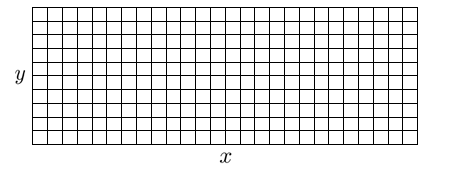
\includegraphics[width= 0.45\textwidth]{./images/map.png}
	\caption{Bisheriges einfaches Raster}
	\label{fig:welt}
\end{figure}
Um dieses Problem zu lösen ist die Idee, dass Raster in Form einer Kugel zu modellieren, so dass die Übergänge weicher werden. Des Weiteren erinnert diese Form eher an die der Erde. Für die Simulationslogik sähe das Raster als Folge dessen wie in Abbildung \ref{fig:kugel} gezeigt aus. Ebenso wären natürliche Hindernisse wie Meere oder ähnliches in der Modellierung denkbar.
\begin{figure}[H]
	\centering
	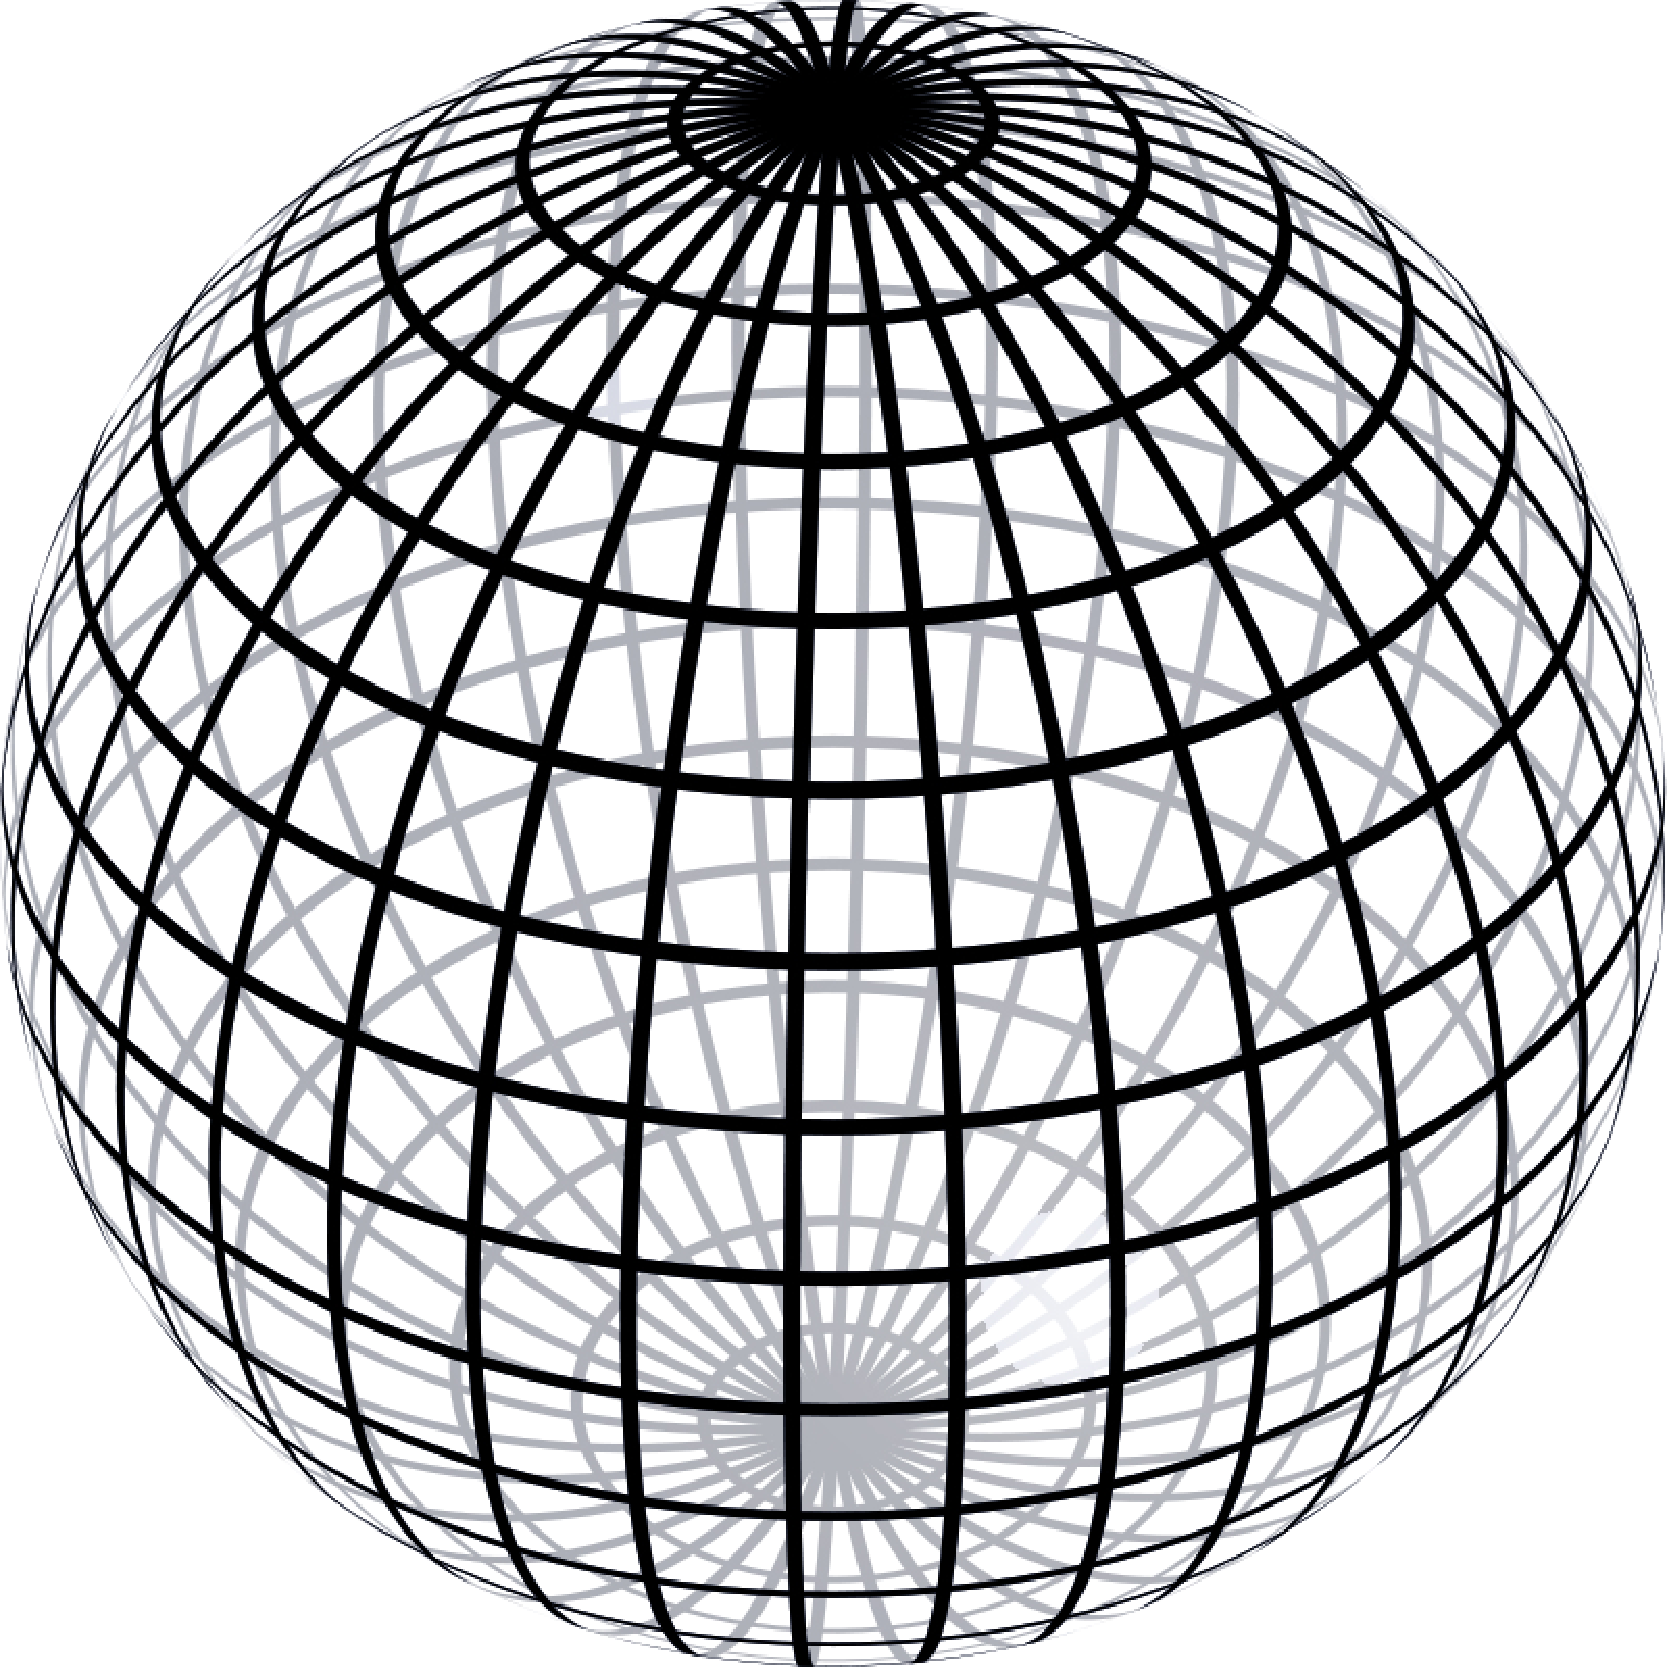
\includegraphics[width= 0.3\textwidth]{./images/kugel.pdf}
	\caption{Raster als Kugel \cite{WikiKugel:2014}}
	\label{fig:kugel}
\end{figure}


Unabhängig davon besteht auch bei der Simulationslogik selbst Verbesserungspotential. Denn ein mögliches Ziel wäre es die Realität bestmöglich auch im Modell abzubilden.
Die Umsetzung von Inkubationszeiten trüge bereits einen enormen Anteil zu diesem Ziel bei. 
Das Problem der Inkubationszeiten lässt sich lösen, indem die Krankheiten weiter spezifiziert werden. Der Zustand der Zellen verändert sich demnach nicht direkt, sondern in Abhängigkeit der Inkubationszeit die bei der Krankheit zu erwarten ist.

Die Zellen, die schon als Objekte existieren, könnten durch weitere Attribute sinnvoll ergänzt werden, damit sie die Realität besser abbilden.
Vor allem Alterung spielt hier ein zentrale Rolle. Das junge widerstandsfähiger als ältere Zellen sind gilt für die meisten Krankheiten, jedoch nicht unbedingt für alle und hängt auch von weiteren Faktoren ab.Das je nachdem bestimmte Zellen anfälliger sind berücksichtigt unser Modell jedoch noch nicht. Ein Lösungsansatz für diese Problem wäre zum einem ein Alter für die Zelle einzuführen als auch die Krankheit mit verschiedenen Wahrscheinlichkeiten für die jeweilige Zielgruppe zu modellieren. 
Durch die Alterung ist  ebenfalls das Problem gelöst, dass Zellen theoretisch ewig leben können, wenn sie keiner Krankheit zum Opfer fallen. 

Dies gilt allerdings nur, wenn zusätzlich eine weitere Voraussetzung erfüllt ist. Die Simulation benötigt eine gewisse Lebenserwartung der Zellen. Diese kann je nach Region oder bisherigen Iterationen variieren und sorgt dafür, dass Zellen nicht ewig leben können.
Zeitgleich wirft diese Lösung ein neues Problem in den Raum und zwar, dass es keine Reproduktion der Zellen gibt. Die Population stürbe auf lange Sicht gesehen aus. Ein möglicher Lösungsansatz wäre hier, mit jeder Iteration eine gewisse Anzahl von neuen Zellen zu erzeugen. Allerdings ist diese Berechnung keineswegs trivial, weil verschiedene Faktoren wie Geschlechterverhältnis, Krankheitsübertragungen während der Schwangerschaft, Überbevölkerung und weitere diese beeinflussen.

Des Weiteren verwendet die Simulation bisher nur die unmittelbare Nachbarschaft. Betrachtet man nun Ballungsgebiete wie New York, Peking oder Tokio ist unmittelbare Nachbarschaft nicht unbedingt ausreichend. Die Wahrscheinlichkeit mit einer Infizierten Person in Kontakt zukommen ist größer als in ländlichen Regionen. Deshalb wäre eine Lösung die Nachbarschaft auszudehnen, so dass weitere Zellen für die Zustände verantwortlich sind. Beispielsweise wie in Abbildung \ref{fig:ewnachbar} gezeigt. Die Moore-Nachbarschaft wird nur auf den Radius 2 erhöht. Die gesunde Zelle in der Mitte hat nun 2 Infizierte Zellen, die für die Berechnung des neuen Zustandes relevant sind. 



An dieser Stelle könnte man zusätzlich eine Art Gauß-Filter verwenden, um auch die Distanz bei der Gewichtung mit einfließen zu lassen. Die Zellen im unmittelbaren Umkreis hätten somit einen größeren Einfluss als diejenigen, die weiter entfernt liegen.
Dafür könnte man 
\begin{center}
 $A = 
\begin{bmatrix}
b & b & b & b & b \\
b & a & a & a & b \\
b & a & 0 & a & b \\
b & a & a & a & b \\
b & b & b & b & b \\
\end{bmatrix}
$ als Faltungsmatrix
\end{center} 
\begin{figure}[t]
	\centering
	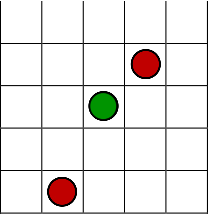
\includegraphics[width= 0.3\textwidth]{./images/ewNachbar.pdf}
	\caption{Augmentierte Nachbarschaft}
	\label{fig:ewnachbar}
\end{figure}
verwenden, um die Distanz mit Faktoren $a,b$ zu gewichten. Beispielsweise könnte man die unmittelbare Nachbarschaft also $a=1$ und die Nachbarschaft mit dem Radius 2 mit $b=\frac{2}{3}$ bewerten. Ebenso könnte man die Diagonale aufgrund höherer Distanz zusätzlich geringer gewichten.

In der vorliegenden Version bewegen sich alle Zellen vollkommen zufällig. Da aber Menschen als auch Tiere sich meist zielgerichtet bewegen, wäre es realistischer anzunehmen dass Zellen einen Zielpunkt auf dem Raster haben oder sich zumindest nicht nach einem Schritt wieder direkt zu ihrer alten Position zurück bewegen. Hier bietet sich beispielsweise das sogenannte \glqq{}Correlated random walks\grqq{}. Bei dem davon ausgegangen wird dass eine Reihe von aufeinanderfolgenden Bewgungen tendziell immer in die Gleiche Richtung geht der Einfluss der vorherigen Bewegungen aber immer weiter abnimmt umso länger sie zurückliegen \cite{Codling:2008}.

Eine weitere Schwachstelle des Modells ist die Verwendung eines Generators von Zufallszahlen. Dieser kann nur pseudo-Zufallszahlen erzeugen welche von der Uhrzeit der Initialisierung in Nanosekunden und der Aufrufe des Generators abhängen \cite{Oracle:2014}. Sollte es also vorkommen das zwei Simulationen zur exakt gleichen Uhrzeit mit den komplett gleichen Parametern gestartet werden, werden sie identische Ergebnisse liefern.\\
Dies könnte man verhindern indem man echte Zufallszahlen aus natürlichen zufälligen Ereignissen ermittelt. Dies tut zum Beispiel die Website \url{http://www.random.org}, diese ermittelt Zufallszahlen aus dem Hintergrundrauschen der Atmosphäre. Eine Einbindung dieses oder eines ähnlichen Services würde obiges beseitigen. Allerdings ist es fraglich ob es bei der Seltenheit bei der das Problem auftritt, überhaupt notwendig ist, sich mit dieser Problematik weiter zu befassen.



\section*{Danksagung}
Wir möchten uns an dieser Stelle bei \emph{Dr. Gerhards} bedanken. Einerseits für die fachliche Hilfe bei diesem Projekt und andererseits für seine hilfreichen Anmerkungen nach der Präsentation im Plenum, die die Basis dieser Ausarbeitung darstellt.\\
Des Weiteren möchten wir uns bei unseren Ausbildungsbetrieben der \emph{SAP SE} und der \emph{ALDI GmbH \& Co. oHG} bedanken ohne die es uns erst gar nicht möglich gewesen wäre an Dr. Gerhards Vorlesung teilzunehmen.



\begin{thebibliography}{99}
\bibitem{gehlhoff2007chronik}
B. Gehlhoff,  \textit{Chronik Jahresrückblick 2006}, 2007,
\url{http://books.google.de/books?id=JtPnf5K1CaIC},
Chronik-Verlag, Seite 15


\bibitem{Spon:2014}Spiegel Online {\it Die Chronologie der BSE-Krise}, 2000, \url{
	http://www.spiegel.de/politik/ausland/rinderseuche-die-chronologie-der-bse-krise-a-105210.html
}, Einsichtnahmen 22.11.2014 10:24


\bibitem{welt:2014}Die Welt {\it Warum die Spanische Grippe so verheerend war} , 2014, \url{http://www.welt.de/gesundheit/article127418306}, Einsichtnahmen 22.11.2014 17:10

	
\bibitem{UNAIDS:2014}UNAIDS {\it FACT SHEET 2014}, 2014,
	\url{http://www.unaids.org/sites/default/files/documents/20141118_FS_WADreport_en.pdf},
	Seite 1, Einsichtnahme 22.11.2014 17:19

	B. Gehlhoff,  \textit{Chronik Jahresrückblick 2006}, 2007,
	\url{http://books.google.de/books?id=JtPnf5K1CaIC},
	Chronik-Verlag, Seite 15



\bibitem{jdmurray}
	J.D. Murray,  \textit{Mathematical Biology: I. An Introduction, Third Edition}, 2002,
	\url{http://www.ift.unesp.br/users/mmenezes/mathbio.pdf},
	Springer-Verlag, Seite 329	


\bibitem{Kesh}
	L. Edelstein-Keshet, \textit{Chronik Jahresrückblick 2006}, 2005,
	\url{http://books.google.de/books?id=uABYP1hnsf0C&printsec=frontcover&hl=de&source=gbs_ge_summary_r&cad=0#v=onepage&q=SIR&f=false},
	SIAM (Society for Industrial and Applied Mathematics), Seite 242-252
	

\bibitem{sebM}
	S. Möhler,  \textit{Ausbreitung von Infektionskrankheiten}, 2004,
	\url{http://www.mathe.tu-freiberg.de/~wegert/Lehre/Seminar3/moehler.pdf}

%Sebastian M¨ohler: Ausbreitung von %Infektionskrankheiten
%Literatur: [2] 242–257, [3] 610–619
	

\bibitem{Weisstein:2014}E. Weisstein {\it Moore Neighborhood}, 2014 \url{http://mathworld.wolfram.com/MooreNeighborhood.html}, Einsichtnahme 22.11.2014 09:14


\bibitem{WikiKugel:2014}Wikipedia {\it Kugel}, \url{http://de.wikipedia.org/wiki/Kugel}, Einsichtnahme 22.11.2014 11:22, mit Änderung übernommen


\bibitem{Codling:2008}E.A. Codling, M.J. Plank und S. Benhamou {\it Random walk models in biology}, 2008; Journal of The Royal Society Interface S. 813-834

\bibitem{Oracle:2014}Oracle  {\it Java Dokumentation: Random},2011; \url{https://docs.oracle.com/javase/6/docs/api/java/util/Random.html}, Einsichtnahme 22.11.2014 19:02
\end{thebibliography}

\end{document}